\documentclass[12pt]{article}
\usepackage{graphicx}
\usepackage{listings}
\usepackage{xcolor}
\usepackage{caption}
\usepackage{subcaption}
\usepackage{amsmath}
\usepackage{geometry}
\geometry{margin=1in}

\title{Lab Report 1: Introduction to Python, NumPy, OpenCV, and Matplotlib}
\author{Tonmoy\\
Roll: 2003027\\
Department of CSE\\
Rajshahi University of Engineering and Technology}
\date{\today}

\definecolor{codegray}{rgb}{0.5,0.5,0.5}
\definecolor{backcolour}{rgb}{0.95,0.95,0.92}

\lstdefinestyle{mystyle}{
    backgroundcolor=\color{backcolour},   
    commentstyle=\color{gray},
    keywordstyle=\color{blue},
    numberstyle=\tiny\color{codegray},
    stringstyle=\color{red},
    basicstyle=\ttfamily\footnotesize,
    breaklines=true,
    captionpos=b,
    keepspaces=true,
    numbers=left,
    numbersep=5pt,
    showspaces=false,
    showstringspaces=false,
    showtabs=false,
    tabsize=2
}

\lstset{style=mystyle}

\begin{document}

\maketitle

\section*{Objective}
The goal of this lab is to introduce students to fundamental programming concepts in Python, array manipulation using NumPy, and image processing using OpenCV and Matplotlib. This also includes understanding color spaces like BGR, RGB, and HSV.

\section*{Tools and Libraries Used}
\begin{itemize}
    \item Python 3.x
    \item NumPy
    \item OpenCV
    \item Matplotlib
\end{itemize}

\section*{Code Explanation}

\subsection*{1. Python Basics: Loops and Arrays}
\begin{lstlisting}[language=Python, caption=Python Loop and NumPy Array]
for i in range(5):
    print(f"Loop iteration: {i}")

array = np.array([1, 2, 3, 4, 5])
print("NumPy Array:", array)

def square_elements(arr):
    return np.square(arr)

squared_array = square_elements(array)
print("Squared Array:", squared_array)
\end{lstlisting}

\subsection*{2. Reading and Displaying Image (BGR vs RGB)}
\begin{lstlisting}[language=Python, caption=Reading and Displaying Image]
image_bgr = cv2.imread('images/image1.jpg')
plt.subplot(1, 2, 1)
plt.imshow(image_bgr)
\end{lstlisting}

\textbf{Note:} OpenCV reads images in BGR color space, which causes colors to appear swapped when displayed using Matplotlib (which uses RGB).

\subsection*{3. Color Space Conversion and HSV Display}
\begin{lstlisting}[language=Python, caption=HSV Conversion and Display]
image_hsv = cv2.cvtColor(image_bgr, cv2.COLOR_BGR2HSV)

cv2.imshow('HSV Image', image_hsv)
cv2.imwrite('output_image_hsv.jpg', image_hsv)
cv2.waitKey(0)
cv2.destroyAllWindows()

plt.subplot(1, 2, 2)
plt.title('HSV Image in Matplotlib')
plt.imshow(image_hsv)
plt.show()
\end{lstlisting}

\textbf{Explanation:} The image is converted from BGR to HSV. OpenCV is used to display and save the image in HSV format. The HSV image is also plotted using Matplotlib for comparison.

\section*{Results and Observations}
\begin{itemize}
    \item Images displayed using OpenCV appear different from those shown using Matplotlib due to BGR vs RGB format mismatch.
    \begin{figure}
        \centering
        \begin{subfigure}[b]{0.45\textwidth}
            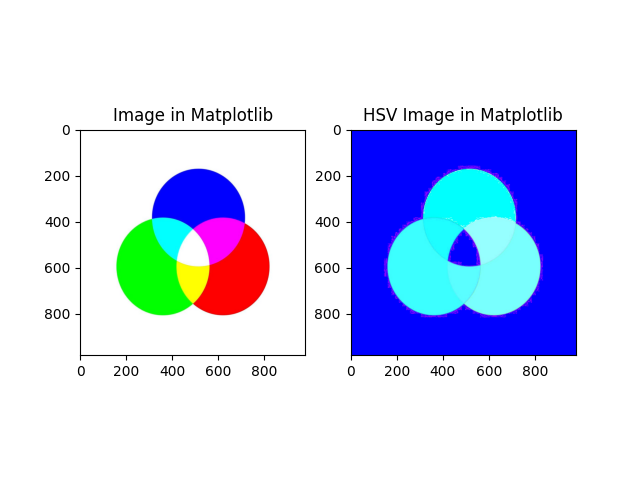
\includegraphics[width=\textwidth]{matplotlib_plots.png}
            \caption{Image displayed using OpenCV (BGR)}
            \label{fig:opencv_bgr}
        \end{subfigure}
        \label{fig:bgr_vs_rgb}
    \end{figure}
    \item Converting to HSV provides better segmentation and color filtering options.
    \item NumPy allows for fast array operations and transformations.
\end{itemize}

\section*{Discussion: BGR vs RGB}
OpenCV uses BGR by default because early standards and camera drivers supported this format more efficiently. Matplotlib, being visualization-focused, follows the RGB convention which aligns with most image viewers and standards.

This leads to color distortion when an OpenCV BGR image is directly shown in Matplotlib without conversion.

\section*{Conclusion}
This lab provided an introduction to Python programming and image processing with OpenCV and Matplotlib. Students learned how to handle loops, arrays, functions, and color space conversions. Understanding the difference between BGR and RGB is crucial when working across different image processing libraries.

\section*{References}
\begin{itemize}
    \item OpenCV Documentation: \texttt{https://docs.opencv.org/}
    \item Matplotlib Documentation: \texttt{https://matplotlib.org/}
    \item NumPy Documentation: \texttt{https://numpy.org/}
\end{itemize}

\end{document}
